\documentclass[a4paper, 12pt, twoside]{article}
\usepackage[utf8]{inputenc}
\usepackage[T1]{fontenc}
\usepackage[francais]{babel}
\usepackage{lmodern}
\usepackage{ae,aecompl}
\usepackage[top=2.5cm, bottom=2cm, 
			left=3cm, right=2.5cm,
			headheight=15pt]{geometry}
\usepackage{graphicx}
\usepackage{float} 
\usepackage{eso-pic}
\usepackage{array} 
\usepackage{hyperref}
\usepackage{enumitem}

\input{pagedegarde}

\title{Vitalys -- Application web de coaching nutrition et sport}
\entreprise{Université Paris Nanterre}
\datedebut{13 mars 2026}
\datefin{22 mai 2026}

\membrea{Ndebi Anaelle -- 45023576}
\membreb{Youssouf Niya -- 45002495}


\begin{document}
\pagedegarde



\newpage

\section*{Remerciements}
Nous tenons à remercier nos enseignants de Licence MIASHS de l'Université Paris Nanterre pour leur aide tout au long du cours d'informatique. Ils nous ont orientées vers les bons outils; Nous remercions également les outils et ressources disponibles en ligne qui nous ont permis d'apprendre et d'avancer tout au long du projet.
\newpage

\tableofcontents
\newpage

\section{Introduction}

Pour notre projet informatique de première année de Licence MIASHS, nous avons créé \textbf{Vitalys}, une application web dédiée au coaching en nutrition et en sport. L'idée est simple : proposer un espace personnel où chaque utilisateur peut suivre son alimentation, recevoir un programme sportif adapté à ses objectifs, et trouver des salles de sport, studios Pilates ou de Yoga en France.

Le site est accessible en ligne à l'adresse : \url{https://vitalys.onrender.com}

Ce rapport explique comment nous avons construit ce projet, les outils que nous avons utilisés, les problèmes que nous avons rencontrés et ce que nous aurions pu améliorer.

\section{Environnement de travail}

Voici les outils que nous avons utilisés pour développer Vitalys :

\begin{itemize}
    \item \textbf{Ordinateur} : MacBook Air sous macOS
    \item \textbf{Éditeur de code} : Visual Studio Code (VS Code) — un logiciel gratuit pour écrire du code
    \item \textbf{Langage de programmation} : Python 3.9
    \item \textbf{Framework web} : Flask — un outil Python qui permet de créer des sites web. Un framework, c'est une boîte à outils qui facilite le développement en fournissant des fonctionnalités prêtes à l'emploi
    \item \textbf{Base de données} : SQLite — un système qui permet de stocker et de retrouver les informations des utilisateurs (leur profil, leurs données de suivi, etc.)
    \item \textbf{Versionnage du code} : Git et GitHub (\url{https://github.com/NdebiAna-code/Vitalys}) — Nous avons utilisé Git et GitHub pour sauvegarder notre code et le mettre en ligne. À la fin du projet, nous avons envoyé l’intégralité de notre code sur GitHub pour pouvoir le déployer sur Render.com    \item \textbf{Hébergement} : Render.com — la plateforme qui met notre site en ligne gratuitement, recommandée par nos enseignants
    \item \textbf{Assistant IA} : Claude (Anthropic) — utilisé pour nous aider à comprendre les messages d'erreur et à trouver des solutions, aussi pour mettre le code au propre , et nous orienter 
    \item \textbf{UptimeRobot} : un outil gratuit qui vérifie notre site toutes les 5 minutes pour qu'il reste toujours actif
    \item \textbf{Photos} : Unsplash — photos gratuites et libres de droits (photos ia)
\end{itemize}

\section{Description du projet et objectifs}

\subsection{Ce que fait Vitalys}

Vitalys est une application web qui permet à un utilisateur de :
\begin{itemize}
    \item Créer un compte personnel et se connecter de façon sécurisée
    \item Renseigner son profil : âge, poids, taille et objectif (perdre du poids, prendre du muscle ou maintenir)
    \item Obtenir son IMC (Indice de Masse Corporelle) calculé automatiquement
    \item Recevoir un plan alimentaire sur 7 jours avec photos de plats, adapté à son objectif
    \item Choisir son type de sport : salle de sport, Pilates, Yoga, ou une combinaison des trois
    \item Accéder à un programme sportif personnalisé selon son choix et son objectif
    \item Trouver des salles de sport, studios Pilates ou Yoga près de chez soi en France
    \item Tenir un journal personnel : noter ses pas quotidiens, prendre en photo ses repas, et suivre l'évolution de son poids
\end{itemize}

\subsection{Ce que ce projet nous a appris}

Ce projet nous a permis d'apprendre à :
\begin{itemize}
    \item Créer un site web complet en Python avec Flask
    \item Gérer une base de données pour sauvegarder les informations des utilisateurs
    \item Mettre en place un système de connexion sécurisé avec mot de passe chiffré
    \item Déployer un site sur internet pour qu'il soit accessible à tout le monde
    \item Utiliser Git et GitHub pour gérer les différentes versions de notre code
\end{itemize}

\section{Bibliothèques, Outils et technologies}

\begin{table}[h]
\begin{center}
\begin{tabular}{|l|l|}
\hline
\textbf{Outil / Technologie} & \textbf{À quoi ça sert} \\
\hline
Flask & Créer le site web en Python \\
\hline
Flask-Login & Gérer la connexion et déconnexion des utilisateurs \\
\hline
SQLite / SQLAlchemy & Sauvegarder les données des utilisateurs \\
\hline
Werkzeug & Chiffrer les mots de passe pour la sécurité \\
\hline
Gunicorn & Lancer le site en ligne sur Render.com \\
\hline
Git / GitHub & Sauvegarder et partager le code \\
\hline
Render.com & Héberger le site sur internet gratuitement \\
\hline
UptimeRobot & Maintenir le site actif en permanence \\
\hline
Unsplash & Photos libres de droits pour illustrer les salles \\
\hline
\end{tabular}
\end{center}

\end{table}

\section{Travail réalisé}

\subsection{Fonctionnalités réalisées}

\begin{itemize}
    \item[\checkmark] \textbf{Système de connexion} : inscription, connexion et déconnexion sécurisées
    \item[\checkmark] \textbf{Profil utilisateur} : formulaire complet avec calcul de l'IMC
    \item[\checkmark] \textbf{IMC intelligent} : si l'IMC indique que la personne est trop mince (IMC inférieur à 18.5), le site refuse l'objectif "perte de poids" et propose un objectif plus adapté
    \item[\checkmark] \textbf{Plan alimentaire} : 7 jours de menus avec photos de plats, selon l'objectif de l'utilisateur
    \item[\checkmark] \textbf{Programme sportif personnalisé} : l'utilisateur choisit entre salle de sport, Pilates, Yoga ou une combinaison des trois
    \item[\checkmark] \textbf{Liste de salles de sport} : plus de 30 lieux vérifiés en France — salles classiques, studios Pilates et studios Yoga
    \item[\checkmark] \textbf{Journal personnel} : compteur de pas quotidien, prise en photo des repas, suivi du poids
    \item[\checkmark] \textbf{Graphique des pas} : histogramme de l'historique des 14 derniers jours
    \item[\checkmark] \textbf{Graphique du poids} : courbe d'évolution du poids semaine par semaine
    \item[\checkmark] \textbf{Mise en ligne} : site accessible publiquement sur \url{https://vitalys.onrender.com}
\end{itemize}

\subsection{Fonctionnalités non réalisées}

\begin{itemize}
    \item[\textbf{$\times$}] \textbf{Photos mensuelles} : nous avions prévu que l'utilisateur puisse uploader une photo de lui chaque mois pour voir son évolution physique. Cela n'a pas été réalisé par manque de temps.
    \item[\textbf{$\times$}] \textbf{Garde-manger intelligent} : l'idée était que l'utilisateur entre les aliments qu'il a chez lui (comme dans un frigo virtuel), et que l'application lui propose des recettes adaptées à son régime alimentaire. Cette fonctionnalité n'a pas été implémentée.
\end{itemize}

\subsection{Répartition du travail}

\begin{table}[h]
\begin{center}
\begin{tabular}{|l|l|}
\hline
\textbf{Tâche} & \textbf{Membre responsable} \\
\hline
Structure du projet et code principal & Ndebi Anaelle \\
\hline
Système de connexion / inscription & Ndebi Anaelle \\
\hline
Calcul IMC et logique de validation & Youssouf Niya \\
\hline
Plans alimentaires et programmes sportifs & Youssouf Niya \\
\hline
Recherche et vérification des adresses de salles & Ndebi Anaelle \\
\hline
Design du site (couleurs, mise en page) & Youssouf Niya \\
\hline
Journal personnel et graphiques & Youssouf Niya \\
\hline
Mise en ligne sur GitHub et Render.com & Ndebi Anaelle \\
\hline
Rédaction du rapport & Ndebi Anaelle et Youssouf Niya \\
\hline
\end{tabular}
\end{center}
\caption{Répartition réelle du travail entre les membres du groupe}
\label{tab:repartition}
\end{table}

\section{Difficultés rencontrées}

Nous avons rencontré plusieurs problèmes au cours du développement. À chaque fois, nous avons cherché des solutions en posant des questions à nos enseignants ou en utilisant l'assistant IA Claude qui nous expliquait les erreurs et nous orientait vers des pistes de résolution.

\begin{enumerate}
    \item \textbf{Nous ne savions pas comment chiffrer les mots de passe} : au début, nous ne savions pas comment faire pour que les mots de passe des utilisateurs soient stockés de façon sécurisée. Claude nous a explique qu'il fallait utiliser un système de chiffrement. Nous avons ensuite rencontré une erreur de compatibilité entre les bibliothèques utilisées et notre version de Python, que Claude nous a aidées à résoudre en changeant les versions.

    \item \textbf{Le site ne se lançait pas en local} : sur macOS, le port 5000  est déjà utilisé par une application Apple appelée AirPlay Receiver. Nous ne comprenions pas pourquoi le site ne s'ouvrait pas. On nous a expliqué l'origine du problème et nous a indiqué d'utiliser un autre numéro de port.

    \item \textbf{Fausses adresses de salles de sport} : au départ, nous avions une liste de 75 salles générée automatiquement. Après vérification sur Google Maps, beaucoup d'adresses étaient incorrectes . Nous avons tout vérifié une par une et avons réduit la liste à environ 30 adresses fiables.

    \item \textbf{La base de données ne se créait pas automatiquement} : la première fois qu'on lançait le site, une erreur apparaissait car les tables de la base de données n'existaient pas encore. Nous avons dû lancer une commande spéciale pour les créer.

    \item \textbf{Nous ne savions pas comment mettre le site en ligne} : on nous ont orientées vers Render.com pour héberger notre site gratuitement. La configuration a nécessité plusieurs essais avant de fonctionner correctement.

    \item \textbf{Le site s'endormait} : sur le plan gratuit de Render.com, le site se met en veille s'il n'est pas visité pendant un moment, ce qui provoquait un délai de 50 secondes à la première ouverture. Claude nous a conseillé d'utiliser UptimeRobot, un outil gratuit qui vérifie le site toutes les 5 minutes pour le maintenir actif en permanence.
\end{enumerate}

\section{Bilan}

\subsection{Conclusion}

Ce projet nous a permis de créer une vraie application web, de A à Z, et de la mettre en ligne. Nous avons appris beaucoup de choses concrètes : comment fonctionne un site web, comment sauvegarder des données, comment sécuriser un espace personnel, et comment déployer un projet sur internet.

Nous avons beaucoup appris en cherchant des solutions aux problèmes rencontrés. L'aide de nos enseignants et de l'outil Claude , chatgpt  a été précieuse, mais nous avons aussi compris qu'il faut toujours vérifier les informations générées automatiquement — comme les adresses des salles de sport qui étaient souvent incorrectes.

Au final, Vitalys est une application fonctionnelle et accessible à tous via \url{https://vitalys.onrender.com}.

\subsection{Perspectives}

Si nous avions plus de temps, voici ce que nous aurions aimé ajouter :

\begin{itemize}
    \item La possibilité d'uploader une photo de soi chaque mois pour voir son évolution physique
    \item Un système de garde-manger : l'utilisateur entre les aliments qu'il a chez lui et reçoit des recettes adaptées à son régime
    \item Des vidéos ou animations pour illustrer les exercices sportifs
    \item Proposer des salles dans davantage de villes en France
\end{itemize}

\newpage
\section{Webographie}

\begin{thebibliography}{4}
   \bibitem[FLASK]{flask} Documentation officielle Flask : \url{https://flask.palletsprojects.com}
   \bibitem[RENDER]{render} Render.com (hébergement) : \url{https://render.com}
   \bibitem[GITHUB]{github} Dépôt GitHub du projet : \url{https://github.com/NdebiAna-code/Vitalys}
   \bibitem[VITALYS]{vitalys} Site Vitalys en ligne : \url{https://vitalys.onrender.com}
\end{thebibliography}

\newpage
\section{Annexes}
\appendix
\makeatletter
\def\@seccntformat#1{Annexe~\csname the#1\endcsname:\quad}
\makeatother

\section{Cahier des charges initial}

Les fonctionnalités prévues au début du projet :
\begin{itemize}
    \item Système de connexion et inscription sécurisé
    \item Calcul IMC avec orientation intelligente selon l'objectif
    \item Plan alimentaire avec photos de plats
    \item Programme sportif avec choix entre salle, Pilates, Yoga ou combinaison
    \item Journal de suivi avec photos mensuelles et compteur de pas
    \item Liste de salles de sport, Pilates et Yoga en France
    \item Garde-manger avec suggestions de recettes selon les ingrédients disponibles
    \item Design vert, noir et blanc 
\end{itemize}

\section{Exemple d'exécution du projet}

\begin{figure}[H]
\centering

\includegraphics[width=0.8\textwidth]{IMG_9830 - Grande.jpeg}
\caption{Page de connexion}
\end{figure}

\begin{figure}[H]
\centering
\includegraphics[width=0.8\textwidth]{IMG_9831 - Grande.jpeg}
\caption{Page d'accueil}
\end{figure}

\begin{figure}[H]
\centering
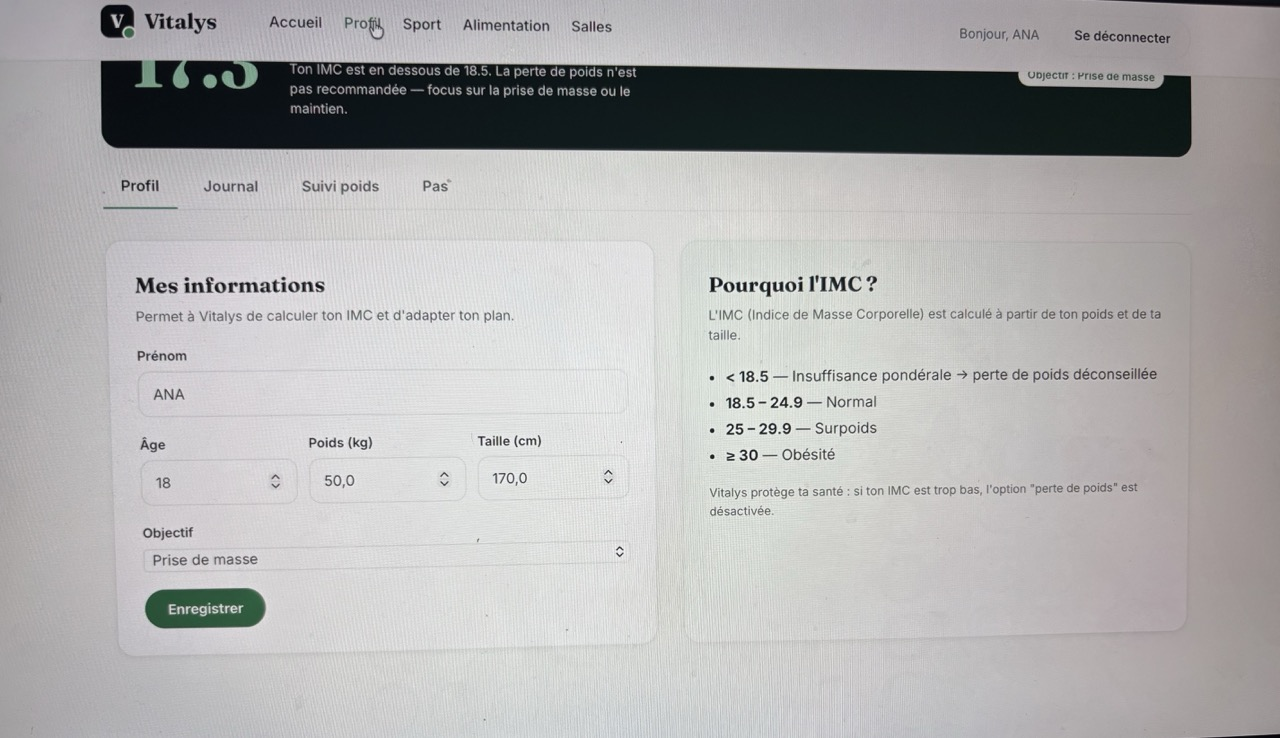
\includegraphics[width=0.8\textwidth]{IMG_9832 - Grande.jpeg}
\caption{Page profil et calcul IMC}
\end{figure}

\begin{figure}[H]
\centering
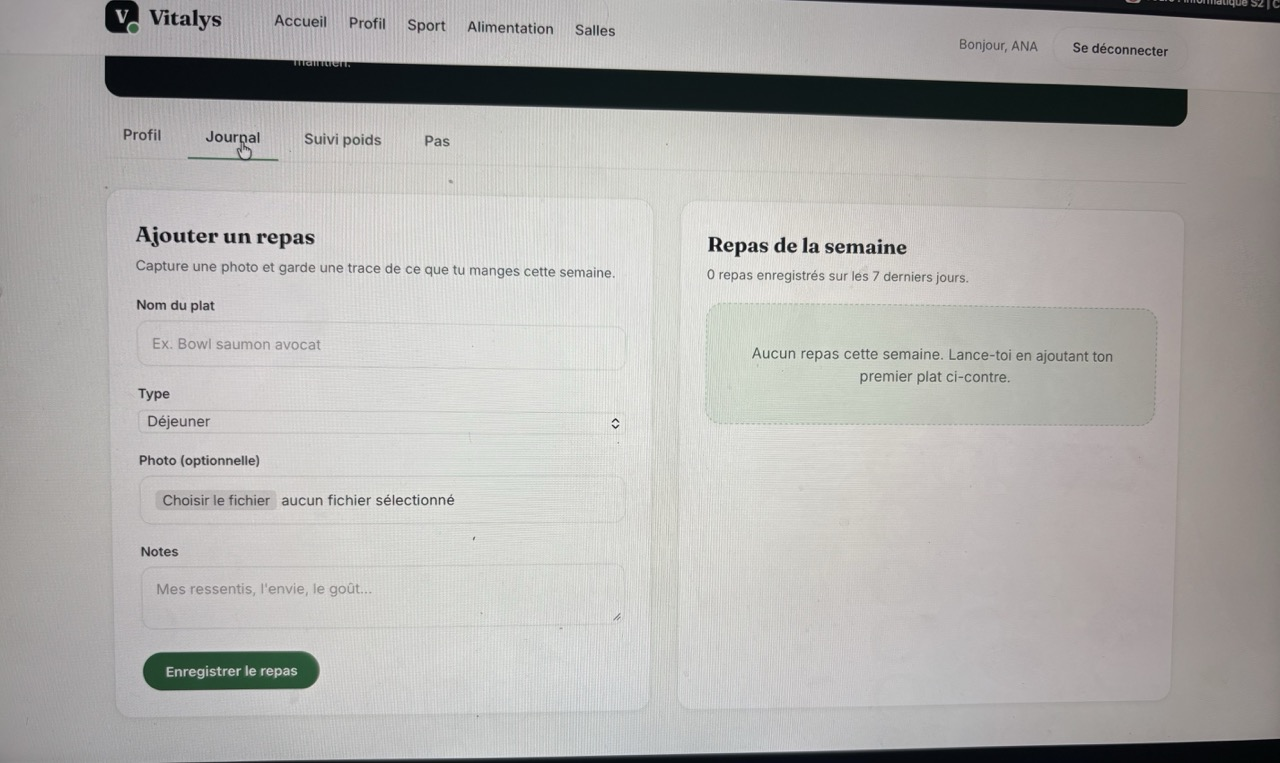
\includegraphics[width=0.8\textwidth]{IMG_9833 - Grande.jpeg}
\caption{Journal alimentaire}
\end{figure}

\begin{figure}[H]
\centering
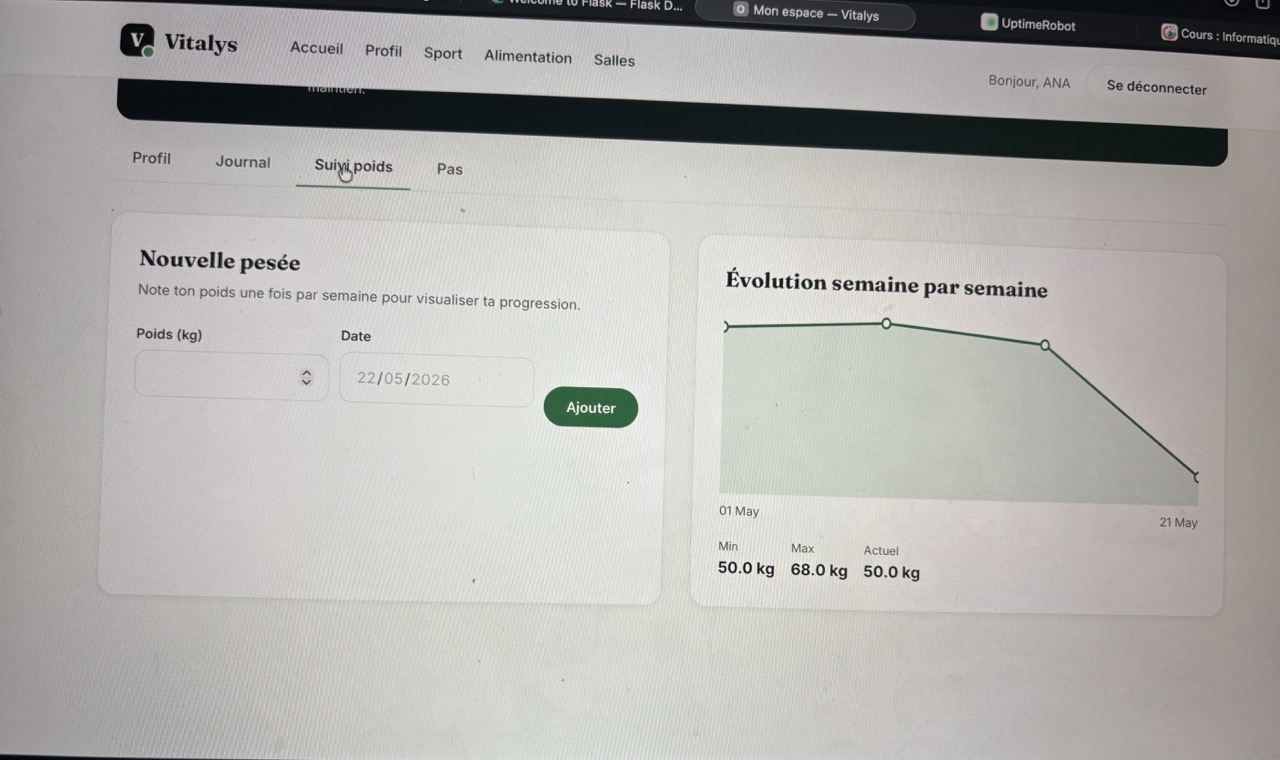
\includegraphics[width=0.8\textwidth]{IMG_9834 - Grande.jpeg}
\caption{Suivi du poids avec graphique}
\end{figure}

\begin{figure}[H]
\centering
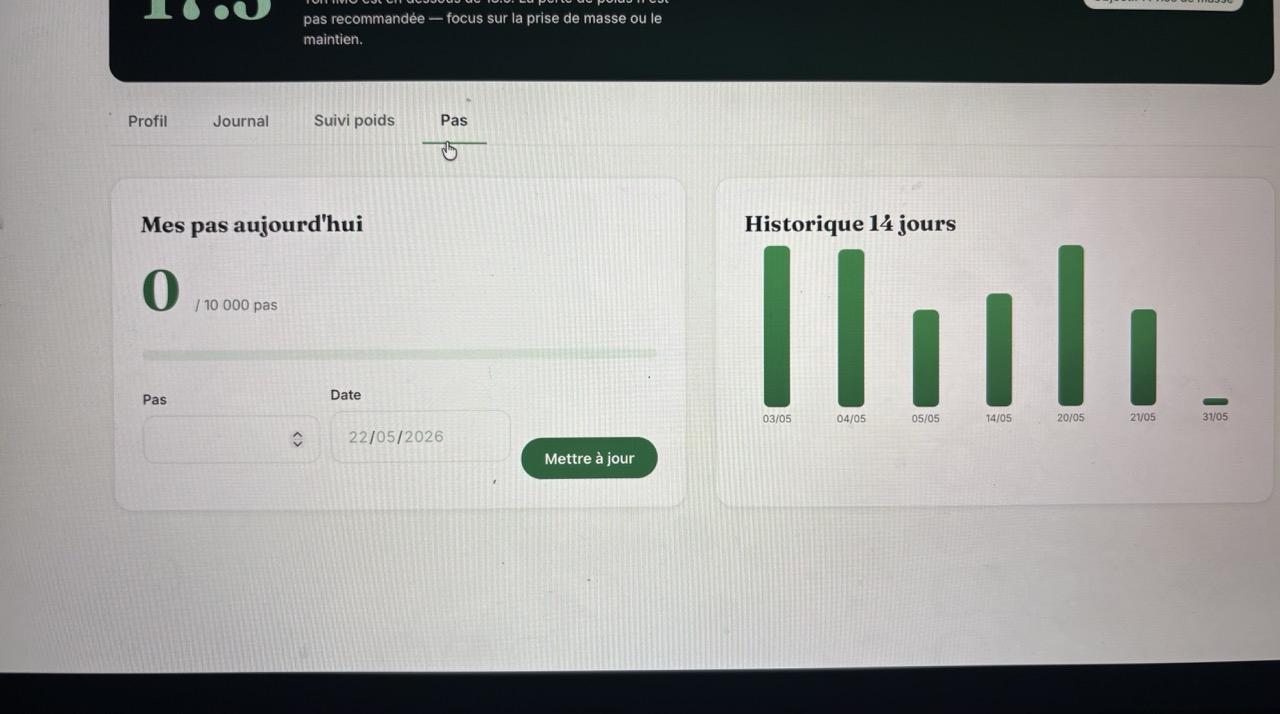
\includegraphics[width=0.8\textwidth]{IMG_9835 - Grande.jpeg}
\caption{Compteur de pas et historique 14 jours}
\end{figure}

\begin{figure}[H]
\centering
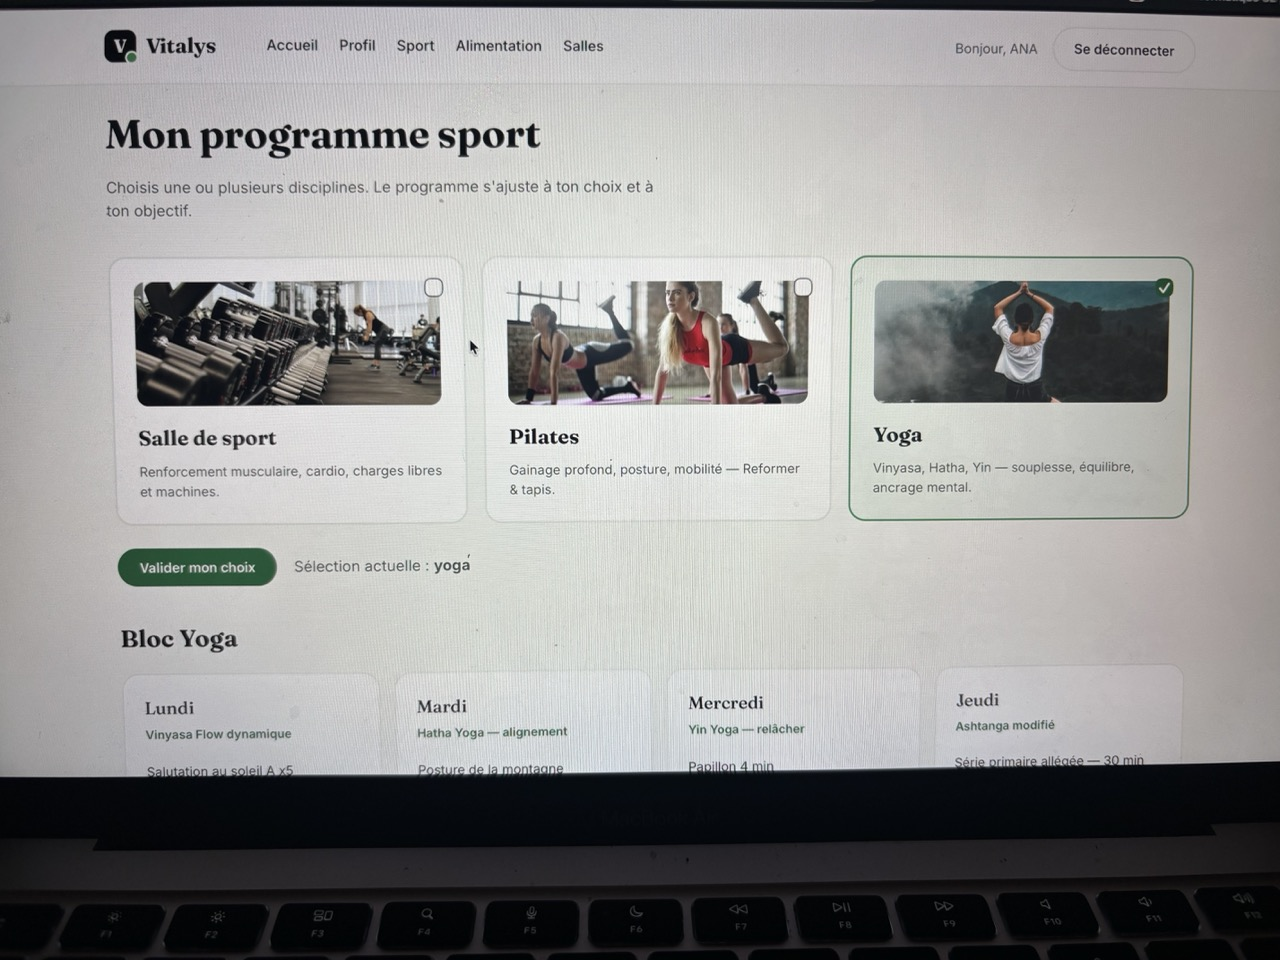
\includegraphics[width=0.8\textwidth]{IMG_9836 - Grande.jpeg}
\caption{Programme sport}
\end{figure}

\begin{figure}[H]
\centering
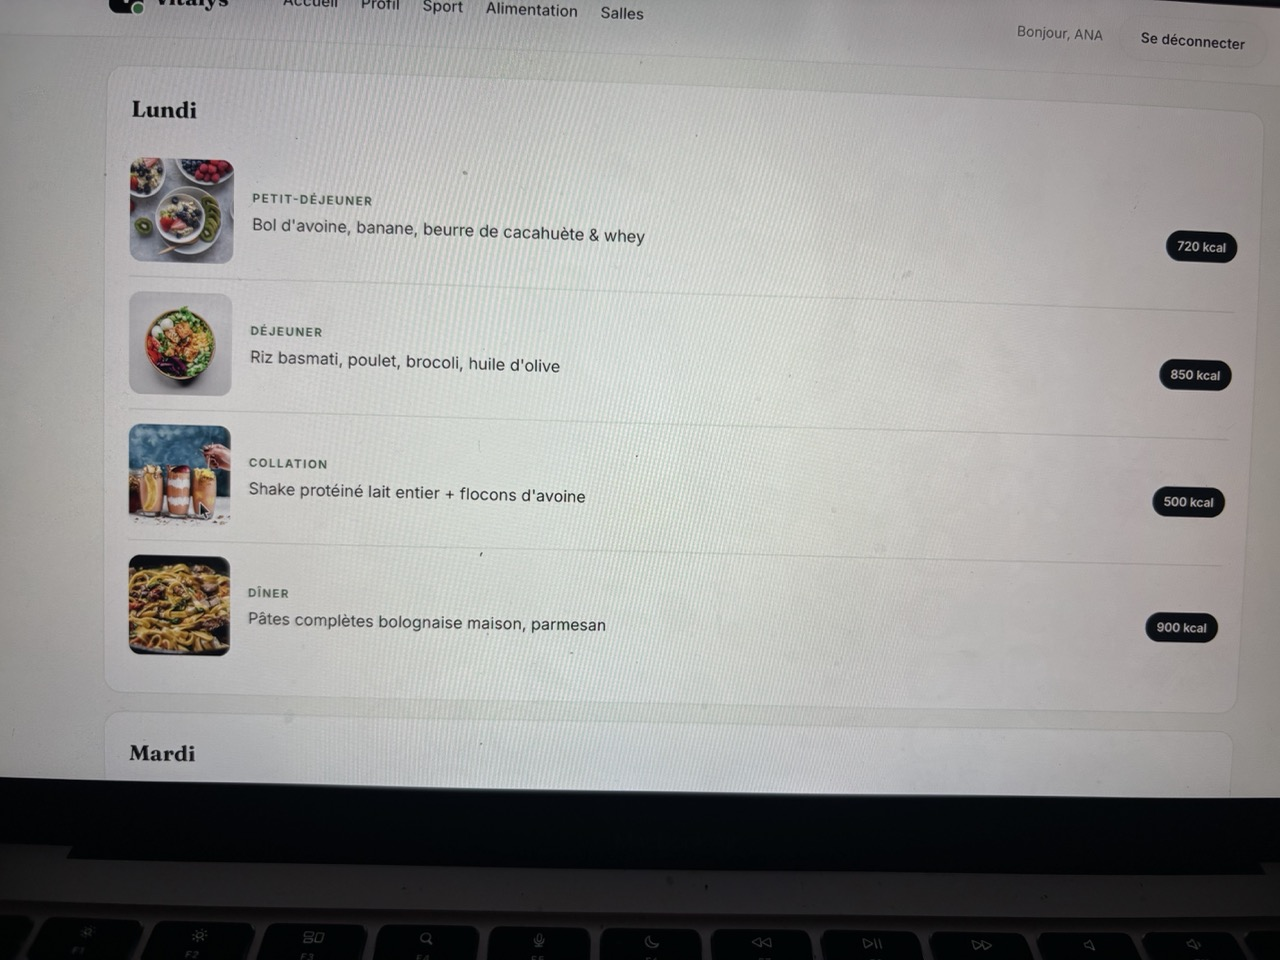
\includegraphics[width=0.8\textwidth]{IMG_9837 - Grande.jpeg}
\caption{Plan alimentaire}
\end{figure}

\begin{figure}[H]
\centering
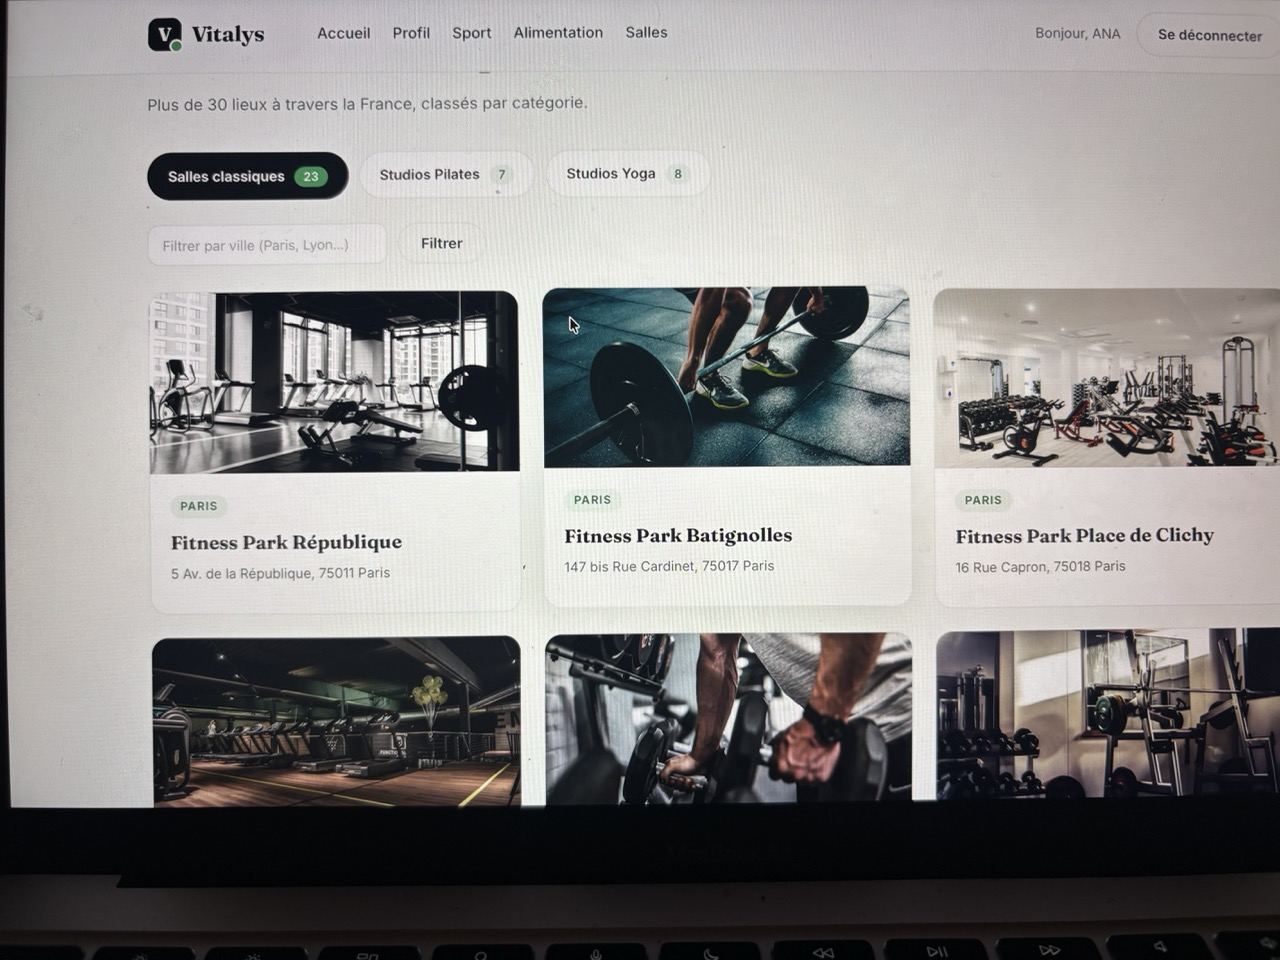
\includegraphics[width=0.8\textwidth]{IMG_9838 - Grande.jpeg}
\caption{Liste des salles de sport}
\end{figure}

Le site en ligne est accessible directement via : \url{https://vitalys.onrender.com}

\section{Manuel utilisateur}

\begin{enumerate}
    \item \textbf{Créer un compte} : cliquer sur "S'inscrire" et renseigner son email et mot de passe
    \item \textbf{Compléter son profil} : renseigner son âge, poids, taille et objectif
    \item \textbf{Consulter son plan alimentaire} : accessible depuis le menu "Alimentation"
    \item \textbf{Accéder à son programme sport} : choisir entre salle, Pilates, Yoga ou combo
    \item \textbf{Trouver une salle} : aller dans "Salles \& studios" et filtrer par ville
    \item \textbf{Tenir son journal} : noter ses pas, prendre ses repas en photo et suivre son poids
\end{enumerate}

\end{document}
